\section{Occlusion, Personalisation and Safe Coaching}\label{sec:occ}
\begin{figure*}[t]
\centering
\begin{subfigure}[t]{0.175\textwidth}\centering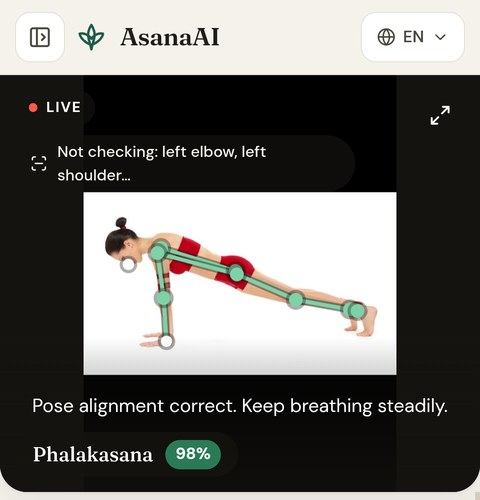
\includegraphics[width=\linewidth]{figures/oc_plank_hidden.jpg}\caption{Hidden joints are not judged}\end{subfigure}\hfill
\begin{subfigure}[t]{0.175\textwidth}\centering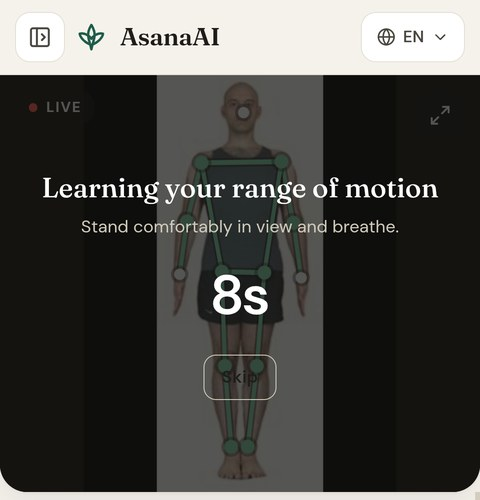
\includegraphics[width=\linewidth]{figures/cal_countdown.jpg}\caption{Calibration: 15\,s countdown}\end{subfigure}\hfill
\begin{subfigure}[t]{0.175\textwidth}\centering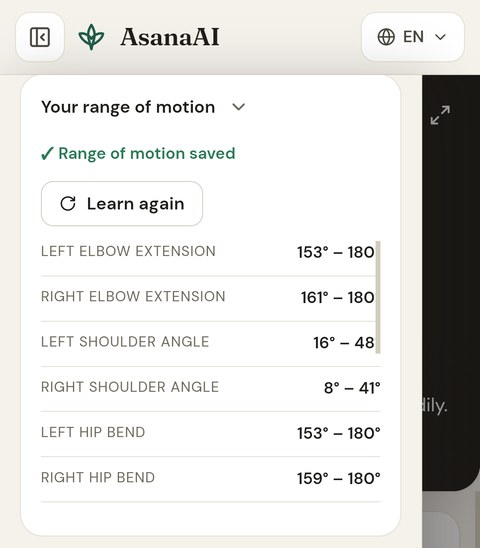
\includegraphics[width=\linewidth]{figures/cal_range.jpg}\caption{Saved range of motion}\end{subfigure}\hfill
\begin{subfigure}[t]{0.175\textwidth}\centering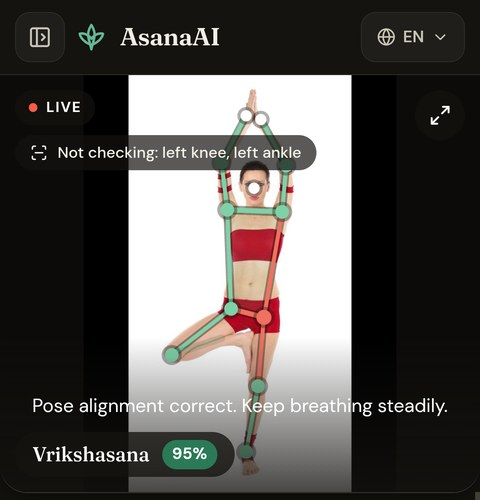
\includegraphics[width=\linewidth]{figures/oc_tree_hidden.jpg}\caption{Failure: false coral leg}\end{subfigure}\hfill
\begin{subfigure}[t]{0.175\textwidth}\centering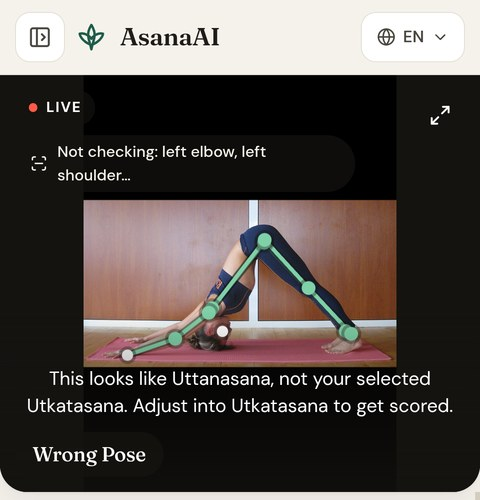
\includegraphics[width=\linewidth]{figures/fail_dog.jpg}\caption{Failure: wrong name}\end{subfigure}
\caption{Live screenshots of the deployed app on a POCO M7 Pro over USB, with a credited Wikimedia photo standing in for the camera (no live person). (a)~Plank, guided mode: visible limbs are sage (inside their angle bands) and the chip ``Not checking: left elbow, left shoulder'' names joints the camera cannot see, which are drawn faint and neither scored nor coached. (b)~Calibration asks the user to stand comfortably for 15\,s. (c)~The learned per-joint ranges are saved on the device (the still photo yields narrow ranges). Two failures shown on purpose: (d)~a correct Tree (guided, dark theme) with a coral standing leg, captured before the fix: Tree has no angle bands, so its joint colours then came from the learned deviation head, which is unreliable; the deployed app now draws neutral limbs for Tree and Lunge (Section~\ref{sec:models}); (e)~a Downward Dog photo named Uttanasana (a forward fold), after which guided mode answers ``Wrong Pose''. Photos: Kennguru (a, d), Witold Fitz-Simon (b, c; CC BY-SA 2.5), Iveto (e); CC BY 3.0 unless noted, via Wikimedia Commons.}
\label{fig:occ}
\end{figure*}

\subsection{Visibility-aware scoring}
An audit of the first version showed that the server's mesh-recovery branch was never wired (nothing sent it data and no such model was deployed), and what actually ran for hidden joints was a left--right mirror: exact for symmetric stances, wrong for asymmetric ones. In Tree pose the raised foot was placed on the floor, off by 0.23 of the frame height, and still reported as ``recovered''. Meanwhile the joint angles were always computed from the raw landmarks, so a hidden joint could still produce a confident wrong score and cue.

We replaced guessing with abstaining. Joints whose landmark visibility is low (smoothed with hysteresis in the browser) are neither scored nor coached; the interface lists what it is not checking (Fig.~\ref{fig:occ}a) and draws hidden limbs at 25\% opacity. The map from hidden joint to affected angle features was checked against the Python angle code by perturbation (0 visibility errors). A known limit remains: the pose name can still be influenced by a hallucinated hidden joint; only scoring and coaching are masked.

\subsection{Would mesh recovery do better? CLIFF versus the mirror}
Mirroring is crude, so we asked whether CLIFF \cite{li2022cliff} (a ResNet-50 model that predicts an SMPL body \cite{loper2015smpl} from the full frame) recovers hidden joints better. On 70 real yoga frames in four poses, with MediaPipe on the clean frame as the reference, a grey box hid one limb (left leg, right arm or both feet; 141 cases) and the hidden joints were recovered four ways. Table~\ref{tab:cliff} gives the errors.
\begin{table}[t]
\centering\footnotesize\setlength{\tabcolsep}{3pt}
\caption{Recovering hidden joints (141 cases; lower is better). Errors are relative to MediaPipe on the clean frame; NME is 2-D distance over torso length. Bold: better of the compared methods within each subset.}\label{tab:cliff}
\begin{tabular}{@{}llrrr@{}}
\toprule
Subset ($n$) & Method & Med.\ angle & Mean angle & Med.\ NME \\ \midrule
All (141) & raw & $17.9^\circ$ & $38.9^\circ$ & 0.291 \\
 & mirror & $8.6^\circ$ & $20.2^\circ$ & \textbf{0.152} \\
 & CLIFF & $\mathbf{5.8^\circ}$ & $\mathbf{16.8^\circ}$ & 0.185 \\
 & CLIFF aligned & $7.0^\circ$ & $22.0^\circ$ & 0.179 \\ \midrule
Symmetric (117) & mirror & $\mathbf{5.2^\circ}$ & $13.8^\circ$ & \textbf{0.131} \\
 & CLIFF & $6.1^\circ$ & $\mathbf{11.0^\circ}$ & 0.173 \\
Tree, asym.\ (24) & mirror & $20.1^\circ$ & $51.2^\circ$ & 0.470 \\
 & CLIFF & $\mathbf{4.8^\circ}$ & $\mathbf{44.8^\circ}$ & \textbf{0.357} \\
Left leg (47) & mirror & $16.2^\circ$ & $33.5^\circ$ & \textbf{0.214} \\
 & CLIFF & $\mathbf{6.2^\circ}$ & $\mathbf{12.7^\circ}$ & 0.270 \\
Right arm (47) & mirror & $\mathbf{4.9^\circ}$ & $\mathbf{11.9^\circ}$ & \textbf{0.092} \\
 & CLIFF & $15.1^\circ$ & $30.7^\circ$ & 0.210 \\
Both feet (47) & mirror ($=$raw) & $6.1^\circ$ & $15.1^\circ$ & 0.199 \\
 & CLIFF & $\mathbf{4.7^\circ}$ & $\mathbf{6.9^\circ}$ & \textbf{0.143} \\ \bottomrule
\end{tabular}
\end{table}
Neither method dominates. The mirror is better where the body really is symmetric (arms, mountain, seated) and has the lowest median landmark error overall; CLIFF is better for legs, for both feet hidden and for the asymmetric Tree pose, and its median joint-angle error is $5.8^\circ$ versus $8.6^\circ$. But CLIFF costs 164\,ms per image on two CPU threads (18.7\,ms on a T4 GPU) and, decisively, needs the image, which the app never sends. We therefore do not ship it and keep the abstain policy. Caveats: 141 cases from 70 frames, one asymmetric pose, a synthetic occluder, a MediaPipe reference rather than motion capture, and a neutral body-model stand-in for an unavailable initialisation file.

\subsection{Personal range-of-motion calibration}\label{sec:calib}
Bodies differ: a joint inside its owner's comfortable range is ``different'', not ``wrong''. At camera start the app offers a 15-second calibration (Fig.~\ref{fig:occ}b): the user stands comfortably in view while the 15 joint angles are recorded. For each joint the profile stores the observed minimum and maximum widened by $15^\circ$ (clamped to $[0^\circ,180^\circ]$) and the mean as the resting angle; if fewer than 20 frames were captured it is discarded rather than ``pretend we calibrated''. The profile lives only in the browser's local storage (Fig.~\ref{fig:occ}c); each request carries the numbers. On the server, a joint whose angle lies inside its personal range has its deviation set to zero, and a personal form score is computed that closes the fraction of the gap to a perfect score that the forgiven deviation represents; it is therefore never lower than the universal score, and equal when nothing is forgiven. The UI shows it as ``For your body'' beside the universal score. We verified the mechanism against the deployed server with a hand-built skeleton (angles from the app's own function; both hip deviations $56^\circ$ from their bands, universal score 0.924). Without a profile the response carries no personal score; a profile not containing the current angles leaves it at 0.924; one containing the left hip's angle zeroes that deviation (0.962); both hips give 1.000; the universal score never changed. A profile spanning $0^\circ$--$180^\circ$ for every joint also gives 1.000, which shows how much a poor profile can forgive. The feature has not been validated with users or clinicians (Section~\ref{sec:limits}).

\subsection{Safe, multilingual coaching}\label{sec:safety}
The cue sentence goes through three stages. (1)~A symbolic stage picks the joint furthest outside its band and a reviewed template for it in English, Hindi or Bengali. (2)~Optionally, a hosted language model (a 27-billion-parameter Qwen model, temperature 0.2) paraphrases the template and may only rewrite it. (3)~A post-generation screen discards the paraphrase and keeps the template if it contains any of ``push'', ``force'', ``hurt'', ``pain'', ``stretch more'' or ``further''. A cue that is delivered and produces no measured improvement escalates: the second time it adds how many degrees off the user is, and from the third time it backs off (``ease out of the shape and reset; come back only as far as feels comfortable today''), because a cue that failed twice usually means the range is not available today. A lesson from operating this stage: when the provider retired the model name we had configured, every request silently fell back to the template and the failure looked identical to success until the response was found to be byte-identical to the template. The fallback is safe, which is exactly why a silent one is dangerous; the code now logs every non-200 answer.
